<%# some convenience definitions %>
<% topdf = (ENV['RB_TOPDF'] || 'pspdf').to_sym %>
<% sonia = @params[:sonia] %>

<%
# We do not want to run TeX more than once, therefore we define \ref:
ref = {
    'sec:statistics' => "#{count = 2}",
    'sub:user_statistics' => "#{count}.1",
    'sub:page_statistics' => "#{count}.2",
    'sec:cumulative_distribution_functions' => "#{count += 1}",
    'sec:revision_history' => "#{count += 1}",
    'sec:author_participation' => "#{count += 1}",
    'sec:network_visualization' => "#{count += 1}",
    'sec:sonia' => "#{count += 1}",
    'fig:cumulative_distribution_functions' => "#{count = 1}",
    'fig:revisions_per_month' => "#{count += 1}",
    'fig:cumulative_revisions_per_month' => "#{count += 1}",
    'fig:number_of_links' => "#{count += 1}",
    'fig:amount_of_text' =>  "#{count += 1}",
    'fig:author_participation' => "#{count += 1}",
    'fig:relative_author_participation' => "#{count += 1}",
    'fig:coauthorship_network' => "#{count += 1}",
    'fig:page_network' => "#{count += 1}",
    'tab:global_statistics' => "#{count = 1}",
    'tab:global_user_statistics' => "#{count += 1}",
    'tab:top-20-users' => "#{count += 1}",
    'tab:top-5-pages' => "#{count += 1}"
  }
%>

<%
# Gnuplot of timeline data
def gp_time(file, title, ylabel, *data)
  topdf = (ENV['RB_TOPDF'] || 'pspdf').to_sym
  Gnuplot.new do |gp|
    gp.set('xdata', 'time')
    gp.set('timefmt', '%Y-%m-%d', true)
    gp.set('format x', '%b %y', true)
    data.each_slice(2) do |array, label|
      gp.add(array, :timefmt => '%Y-%m-%d',
             :with => 'lines', 
             :title => label )
    end
    gp.set('xtics rotate')
#    gp.set("title \"#{title}\"")
#    gp.set('xlabel "month"')
    gp.set("ylabel \"#{ylabel}\"")
    gp.plot(topdf => file, :range => '[][0:]')
  end 
end
%>

<%
wiki = @wiki
full = wiki.filter.clone; full.include_all_namespaces
ufilter = full.clone
ufilter.deny_anons = true
ufilter.deny_user(0)
# Set Filter and Time Raster
filter = full.clone # clone filter
filter0 = full.clone
filter0.namespace = 0
sfilter = filter.clone
sfilter0 = filter0.clone

allpages = wiki.pages(full).to_a
allpages0 = wiki.pages(filter0).to_a

allrevisions = wiki.revisions(full).to_a

users = wiki.users(ufilter).to_a

wn = wiki.name.tr(' ','_')

ns_default = {}
NS_Default_Mapping.each { |k,v| 
  ns_default[v] = k.gsub(/_/, '\_') if k.kind_of?(String) }
ns_default[NS_PROJECT] = 
  NS_Default_Mapping[:project].gsub('%', wn).gsub(/_/, '\_')
ns_default[NS_PROJECT_TALK] = 
  NS_Default_Mapping[:project_talk].gsub('%', wn).gsub(/_/, '\_')
ns_lang = ns_default.clone
nsl=false
nsl = NS_Mappings[wiki.language]
if nsl
  nsl.each { |k,v| ns_lang[v] = k.gsub(/_/, '\_') if k.kind_of?(String)}
  if p = nsl[:project]
    ns_lang[NS_PROJECT] = p.gsub('%', wn).gsub(/_/, '\_')
  end
  if p = nsl[:project_talk]
    ns_lang[NS_PROJECT_TALK] = p.gsub('%', wn).gsub(/_/, '\_')
  end
end


ns_pages = Hash.new(0)
ns_revs = Hash.new(0)
allpages.each { |p| 
  ns = p.namespace
  ns_pages[ns] +=1 
  ns_revs[ns] += p.revisions(full).length
}

# set time raster to spells of 4 weeks
raster = wiki.timeraster(:zero => :week, :step => 28*24*3600) 

# events
events = users.collect{ |u| 
	[ u.time_of_first_event, u.time_of_last_event ] 
    }.select { |f,l| f && l }

#crpw = raster[1..-2].collect { |e| filter.endtime = e 
#  [ e, wiki.revisions(filter).length ]
#}

aupart = []
aurel = []
rpw = []
lpw = []
tpw = []
rpw0 = []
lpw0 = []
tpw0 = []
raster[1..-2].each_cons(2) { |s,e| 
  filter.revision_timespan = (s..e)
  filter0.revision_timespan = (s..e)
  sfilter.endtime = e
  sfilter0.endtime = e
  pages = wiki.pages(sfilter).to_a # should be faster
  pages0 = wiki.pages(sfilter0).to_a # should be faster
  rpw << [ e, wiki.revisions(filter).length ]
  rpw0 << [ e, wiki.revisions(filter0).length ]
#  nodesl = wiki.coauthorgraph(filter).remove_lonely_nodes.nodes.length.to_f
  awe = 0.0
  users.each { |u| awe += 1 if u.revisions(filter).length > 0 }
  aupart << [ e, awe ]
  # The following could be done more efficiently:
  aurel << [ e, awe / 
                events.reject { |f,l| (f > e) || (l < s) }.length ]
  # I learned inject is expensive (at least in ruby 1.8), so i do it
  # by hand:
  s=0; allpages.each { |p| s+= p.links(sfilter).length }
  lpw << [e, s]
  s=0; allpages0.each { |p| s+= p.links(sfilter0).length }
  lpw0 << [e, s]
  s=0; pages.each { |p| 
    if r=p.revision(sfilter)
      s+= r.size
    end }
  tpw << [e, s]
  s=0; pages0.each { |p| 
    if r=p.revision(sfilter0)
      s+= r.size
    end }
  tpw0 << [e, s]
}
s = 0; crpw = rpw.collect { |e,i| [e,s+=i] }
s = 0; clpw = lpw.collect { |e,i| [e,s+=i] }
s = 0; crpw0 = rpw0.collect { |e,i| [e,s+=i] }
s = 0; clpw0 = lpw0.collect { |e,i| [e,s+=i] }

%>


\documentclass{scrartcl}

\usepackage[T1]{fontenc}
\usepackage{lmodern}
\usepackage{ccfonts}
\usepackage[utf8]{inputenc}
\usepackage{german}
\usepackage{booktabs}
\usepackage{tabularx}
\usepackage{graphicx}
%\usepackage{subfigure}
\usepackage{url}
<% if sonia %>
\usepackage{textcomp}
\usepackage{attachfile}
<% end %>

\newcommand{\todo}{\textcolor{red}}

\renewcommand\floatpagefraction{.7}
\renewcommand\topfraction{.8}
\renewcommand\bottomfraction{.3}
\renewcommand\textfraction{.2}



\title{Mediawiki Report -- <%= wiki.to_s %>
}
\author{Wiki Explorator\footnote{\protect\url{http://wiki-explorator.rubyforge.org}}}

\begin{document}
\maketitle

\section{Einführung} % (fold)
\label{sec:introduction}

Ein Wiki entwickelt sich mit der Zeit. Mehr und mehr Autoren beteiligen sich, editieren und erstellen mehr und mehr Seiten und das Wiki wächst. Das kann man aufgrund der History zeigen. Einige statistische Maße und Visualisierungen der momentanen Struktur sollen im Folgenden vorgestellt werden.

Dies ist eine automatische Auswertung der Struktur ihres Wikis. Kapitel~<%=ref['sec:statistics']%>
liefert einige statistischen Maße über das Wiki als Ganzes und über die einzelnen Wiki-Nutzer (Abschnitt~<%=ref['sub:user_statistics']%>) 
und Wiki-Seiten (Abschnitt~<%=ref['sub:page_statistics']%>).
Das vermittelt Ihnen einen allgemeinen Eindruck davon, was in Ihrem Wiki passiert. 
Kapitel~<%=ref['sec:cumulative_distribution_functions']%>  
zeigt kumulative Verteilungsfunktionen des Wikis, die Aussagen wie „20\% der Nutzer erledigen 80\% der Arbeit.“ erlauben. Kapitel~<%=ref['sec:author_participation']%>
beschreibt die Änderungen der Wiki-Seiten in der Zeit, Kapitel~<%=ref['sec:network_visualization']%>  
macht das Gleiche für die Autoren. Kapitel~<%=ref['sec:network_visualization']%> 
schließlich zeigt verschiedene  Visualisierungen Ihres Wikis, insbesondere das Hyperlink-Netzwerk und das Koautoren-Netzwerk.
<% if sonia %>
Die SoNIA-Datei zur animierten zeitlichen Darstellung findet sich in Kapitel~<%=ref['sec:sonia']%>.
<% end %>

\section{Statistiken} % (fold)
\label{sec:statistics}


\begin{table}
  \centering
  \caption{Allgemeine Wiki-Statistiken}\vspace{0.2ex}

  \label{tab:global_statistics}

  \begin{tabular}{>{\bfseries}lrrr}\toprule
    Namespace && \#pages & \#revisions\\
    \midrule
<% ns_pages.keys.sort.each do |ns| %>
      <%if ns==0 %>
        \textit{main}
      <%else%>
        <%=ns_lang[ns]%>
      <%end%> & (<%=ns%>) & <%=ns_pages[ns]%> & <%=ns_revs[ns]%>\\
<%end%>
    \midrule
    total && <%=s=0;ns_pages.values.each {|i| s+=i};s%> 
    & <%=s=0;ns_revs.values.each {|i| s+=i};s%>\\\bottomrule
  \end{tabular}
  \vspace{1ex}

  \caption{Allgemeine Nutzerstatistiken}\vspace{0.2ex}

  \label{tab:global_user_statistics}
  \begin{tabular}{>{\bfseries}lrrrrr}\toprule
    &\textbf{mean} &\textbf{s.\,d.} &\textbf{median} &\textbf{min.}
    &\textbf{max.}\\
    \midrule
<%=
wiki.global_userstats(ufilter).collect { |a|
  a.collect { |v| 
    if v.nil?
      '-/-'
    elsif v.kind_of?(String)
      v
    elsif v.integer? 
      '%5i' % v
    elsif v.nan?
      '---'
    else
      '%7.2f' % v
    end
  }.join('&')
}.join('\\\\')
    %>
\\\bottomrule
  \end{tabular}
\end{table}



Für diejenigen, die mit Wikis nicht vertraut sind, führen wir kurz
einige der gängigsten Begriffe ein. Ein Wiki besteht aus \emph{Seiten} oder
\emph{Artikeln}, die der Reihe nach von Nutzern bzw. Autoren geschrieben
werden. Jedes Mal, wenn ein Nutzer eine Seite bearbeitet
(z.\,B. erstellt oder verändert), wird eine neue Revision (Version) zur
Revision History (Versionsgeschichte) hinzugefügt.

Die Seiten sind in Namensräumen angeordnet. Normale Seiten
(z.\,B. Artikel) gehören zum Hauptnamensraum (Namespace 0). Es gibt
Namensräume für persönliche Nutzerseiten (eingeleitet von dem Präfix „<%=d=ns_default[2]%>:“<% if (p=ns_lang[2]) != d  %>, or „<%=p%>:“<% end%>),
Hilfeseiten (Präfix „<%=d=ns_default[12]%>:“<% if (p=ns_lang[12]) != d  %>, or „<%=p%>:“<% end%>)
und andere.
Jede Seite kann eine dazugehörige Diskussionsseite (Präfix: „<%=d=ns_default[1]%>:“<% if (p=ns_lang[1]) != d  %>, or „<%=p%>:“<% end%>
für den Hauptnamensraum, „<%=d=ns_default[3]%>:“<% if (p=ns_lang[3]) != d  %>, or „<%=p%>:“<% end%>
für Nutzerdiskussionsseiten und so weiter) haben.



Da jede Revision das Ergebnis einer einzigen Bearbeitung eines einzelnen Nutzers ist, wissen wir \emph{wer} etwas zu \emph{welcher} Seite beigetragen hat -- vorausgesetzt der Nutzer ist eingeloggt. Wenn das Wiki anonyme Bearbeitungen erlaubt, ist keine Abbildung der Nutzer möglich. Anonyme Bearbeitungen erkennt man daran, dass statt des Nutzernamens die IP-Adresse des benutzten Computers angegeben ist. Private Internet Service Provider (ISPs) weisen einem Computer jedes Mal eine andere IP-Adresse zu, wenn er sich in das Internet einwählt, somit sind diese Nutzer nicht eindeutig identifizierbar. Daher schließen wir anonyme Nutzer in nutzerabhängigen Statistiken aus. Ebenso schließen wir den Systemnutzer aus, der als Autor von Default- und automatisch erstellten Seiten aufgeführt wird. 


Ihr Wiki hat zur Zeit <%=allpages.length%> 
Seiten mit insgesamt <%=allrevisions.length%> 
Änderungen und es gibt <%=users.length%> 
nicht-anonyme Nutzer. Tabelle~<%=ref['tab:global_statistics']%> 
gibt einen detaillierteren Überblick.

\subsection{Nutzerstatistiken} % (fold)
\label{sub:user_statistics}

Tabelle~<%=ref['tab:global_user_statistics']%> 
führt die Statistiken der Nutzer im gesamten Wiki auf. Die meisten dieser Statistiken bedürfen keiner weiteren Erklärungen. So zeigt beispielsweise der Durchschnittswert (mean) der Bearbeitungen wie viele Bearbeitungen ein einzelner Nutzer im Schnitt vornimmt. Die Standardabweichung (standard deviation, s.\,d.), der Median, das Minimum (min.) und das Maximum (max.) sind ebenfalls Maße für die Anzahl der Bearbeitungen (Edits), bearbeitete Seiten sowie Edits je Seite. Die Statistiken für Selbst-Edits und Fremd-Edits hingegen benötigen einige Erläuterungen. 
Bei einem Selbst-Edit speichert der gleiche Autor eine Seite mehrmals hintereinander, dies beschreibt aufeinanderfolgende Bearbeitungen von ein und demselben Autor auf einer einzelnen Seite. Vor allem Autoren, die häufig zwischenspeichern, haben hier hohe Werte. Im Gegensatz dazu sind Fremd-Edits zwei aufeinanderfolgende Bearbeitungen unterschiedlicher Nutzer auf einer einzigen Seite. Diese zeigen dann die Zusammenarbeit auf einer Seite an. 
%anderer Begriff für Fremd-Edits (reziproke Edits?)

Tabelle~<%=ref['tab:top-20-users']%> 
führt die Top 20 Nutzer auf, geordnet nach der Anzahl ihrer Edits. %wo stehen die Nutzer in der Tabelle?
Desweiteren kann man ihr die Anzahl der bearbeiteten Seiten, Edits pro Seite, Selbst-Edits und Fremd-Edits entnehmen. Allgemein kann man sagen, dass Nutzer mit vielen Edits auch dazu tendieren, viele Seite zu bearbeiten. Das trifft besonders bei vielen Fremd-Edits zu, da es sehr wahrscheinlich ist, dass sich die Zusammenarbeit über mehrere Seiten erstreckt. %richtig verstanden?


\begin{table}
  \centering
  \caption{Top 20 Nutzer}
	\label{tab:top-20-users}
  \begin{tabular}{rrrrr}\toprule
    \textbf{\#edits} & \textbf{\#pages} &
    \textbf{edits/page} & \textbf{\#self edits} & \textbf{\#foreign
  edits}\\
\midrule
<%= 
wiki.userstats(ufilter).sort_by { |u,v| -v.first }[0...20].collect { |u,values| 
  (values[0..4].collect { |v|
     if v.kind_of?(String)
       v
     elsif v.integer? 
       '%5i' % v
     elsif v.nan?
       '---'
     else
       '%7.2f' % v
     end
   }).join('&')
}.join('\\\\')
%>
\\\bottomrule
\end{tabular}
\end{table}

% subsection user_statistics (end)

\subsection{Seitenstatistiken} % (fold)
\label{sub:page_statistics}

Tabelle~<%=ref['tab:top-5-pages']%> 
listet die Top 5 Seiten jeweils jeweils in Bezug auf die Anzahl ihrer Edits, Nutzer, ausgehende Links (links$\rightarrow$, auch „outdegree“), auf die Seite verweisende Links ($\rightarrow$links, auch „indegree“), und Textgröße (in Bytes). Auch diese Statistiken sprechen für sich selbst.

<%
destlinks = Hash.new(0)
allpages.each { |p| p.links.each { |q| destlinks[q] += 1 } }
# number of pages
n=5
pagelist = allpages.collect { |p| 
  r = p.revision
  ns = p.namespace
  [(ns == 0) ? p.title : p.title + "~(#{ns})",
   p.users.length, p.revisions.length,
   p.links.length, destlinks[p], r ? r.length : 0] }
p_hubs   = pagelist.sort_by { |t,u,r,s,d,l| -s }[0...n]
p_dests  = pagelist.sort_by { |t,u,r,s,d,l| -d }[0...n]
p_revs   = pagelist.sort_by { |t,u,r,s,d,l| -r }[0...n]
p_users  = pagelist.sort_by { |t,u,r,s,d,l| -u }[0...n]
p_size   = pagelist.sort_by { |t,u,r,s,d,l| -l }[0...n]

def p_table(array, txt)
  "\\midrule
\\textit{#{txt}}&&&&&\\\\
\\midrule
#{array.collect { |a|
  '%s & %i & %i & %i & %i & %i' % a
}.join('\\\\')}"
end
%>

\begin{table}
  \centering\small 
  \caption{Top 5 Seiten}
	\label{tab:top-5-pages}
  \begin{tabularx}{\linewidth}{Xrrrrrr}\toprule
    \textbf{title} & \textbf{\#users} &\textbf{\#edits} 
    &\textbf{\#links$\rightarrow$} &\textbf{\#$\rightarrow$links}
    &\textbf{size}\\
    <%=p_table(p_revs, 'by edits') %>\\
    <%=p_table(p_users, 'by users') %>\\
    <%=p_table(p_hubs, 'by outgoing links') %>\\
    <%=p_table(p_dests, 'by incoming links') %>\\
    <%=p_table(p_size, 'by text size') %>\\
    \bottomrule
  \end{tabularx}
\end{table}

% subsection page_statistics (end)

% section statistics (end)

%%% Cumulative Distribution Functions: Lorenz, Gini, Pareto %%%

\section{Kumulative Verteilungsfunktionen} % (fold)
\label{sec:cumulative_distribution_functions}

% Authors vs. Revisions
<%
ur = users.collect { |u| u.revisions(full).length }
ur.gp_plot_lorenz(:title => "Lorenz Curve", :xlabel => "authors", :ylabel => "revisions", topdf => 'cdfar.pdf')
%>

% Authors vs. Pages
<%
up = users.collect { |u| u.pages(full).length }
up.gp_plot_lorenz(:title => "Lorenz Curve", :xlabel => "authors", :ylabel => "pages", topdf => 'cdfap.pdf')
%>

% Revisions vs. Pages
<%
pr = allpages.collect { |p| p.revisions(full).length }
pr.gp_plot_lorenz(:title => "Lorenz Curve", :xlabel => "pages", :ylabel => "revisions", topdf => 'cdfpr.pdf')
%>

\begin{figure}
  \centering
  \begin{tabular}{@{}ccc@{}}
    \includegraphics[width=0.3\textwidth]{cdfar} &
    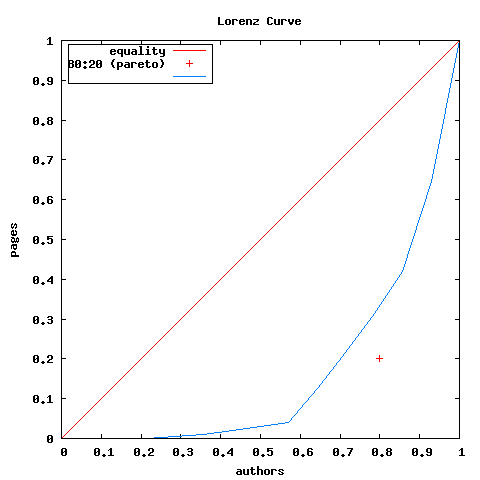
\includegraphics[width=0.3\textwidth]{cdfap} &
    \includegraphics[width=0.3\textwidth]{cdfpr}\\
    Autoren vs. Revisionen &
    Autoren vs. Seiten &
    Revisionen vs. Seiten
  \end{tabular}
  \caption{Kumulative Verteilungsfunktion (Lorenzkurve)}
  \label{fig:cumulative_distribution_functions}
\end{figure}

Abbildung~<%=ref['fig:cumulative_distribution_functions']%> 
zeigt drei kumulative Verteilungsfunktionen (Lorenzkurve), jeweils eine für jede möglich Zusammensetzung von Autoren, Seiten und Revisionen.
Für nähere Erläuterungen betrachten wir den Graphen, der  Autoren zu Revisionen ins Verhältnis setzt. Das rote Kreuz markiert den Punkt des \emph{Paretoprinzips}. Dieses, auch bekannt als „80-zu-20-Regel“, besagt, dass bei vielen Ereignissen grob geschätzt 80\,\% der Wirkung aus 20\,\% der Ursachen resultieren (z.\,B. verfügen 20\,\% der Bürger einer Nation über 80\,\% ihres Reichtums). Auf das Wiki übertragen, bedeutet dies, dass etwa 80\,\% aller Revisionen von 20\,\% der Autoren vorgenommen werden. Liegt die Verteilungskurve unter dem \emph{„Pareto-Punkt“}, lässt dies darauf schließen, dass Ihr Wiki von sehr wenigen Leuten unterhalten wird. Auch wenn dies ein unerwünschter Zustand ist, muss man ihn unter dem Gesichtspunkt der absoluten Autorenanzahl betrachten. So werden z.\,B. in der deutschen Wikipedia nahezu 80\,\% der Revisionen von 2\,\% (!) der mehr als hunderttausend Autoren getätigt.


% section cumulative_distribution_functions (end)

\section{Revision History} % (fold)
\label{sec:revision_history}

<% 
gp_time('rpw.pdf', 'Revisions per Month', 'number of revisions', 
        rpw, 'all', rpw0, 'namespace 0')
gp_time('crpw.pdf', 'Cumulative Revisions per Month', 
        'cumulative number of revisions',
        crpw, 'all', crpw0, 'namespace 0')
%>
\begin{figure}
	\centering
	\includegraphics[width=0.95\textwidth]{rpw}
	\caption{Revisionen pro Monat}
	\label{fig:revisions_per_month}
        \vfill

	\includegraphics[width=0.95\textwidth]{crpw}
	\caption{Kumulative Revisionen pro Monat}
	\label{fig:cumulative_revisions_per_month}
\end{figure}

<% 
gp_time('lpw.pdf', 'Number of Links', 'number of links', 
        lpw, 'all', lpw0, 'namespace 0')
%>
<% 
gp_time('tpw.pdf', 'Amount of Text', 'text (in bytes)', 
        tpw, 'all', tpw0, 'namespace 0')
%>
\begin{figure}
	\centering
	\includegraphics[width=0.95\textwidth]{lpw}
	\caption{Anzahl der Links}
	\label{fig:number_of_links}

	\includegraphics[width=0.95\textwidth]{tpw}
	\caption{Textgröße (in Bytes)}
	\label{fig:amount_of_text}
\end{figure}

Die Abbildungen~<%=ref['fig:revisions_per_month']%> 
und 
<%=ref['fig:cumulative_revisions_per_month']%> 
stellen die absolute und kumulative Anzahl der Revisionen pro Monat dar, jeweils für den Hauptnamensraum und insgesamt. Das zeigt zum Einen, wie viel Arbeit hier monatlich geleistet wird, zum Anderen gibt es einen Überblick über das Wachstum Ihres Wikis. Sie sollten jedoch beachten, dass die Anzahl der Revisionen nicht auf den Inhalt schließen lässt. Auch eine Seite mit wenig Revisionen kann viel Inhalt haben. Jedoch weisen viele Revisionen auf eine aktive Nutzung Ihres Wikis hin, was zur Folge hat, dass sein Inhalt auf dem neuesten Stand ist. 

In beiden Abbildungen sind häufig Ferien und Feiertage (Weihnachten, Sommerferien, etc.) erkennbar, da ein Wiki in diesen zeiten häufig anders (je nach Wiki-Art stärker oder weniger) genutzt wird. Falls sie je versucht haben, ihr Wiki „anzuschubsen“ oder „Starthilfe zu geben“, sollten sich auch diese Ereignisse in den Graphiken anhand vieler Revisionen wieder spiegeln.

% section revision_history (end)

\section{Autorenbeteiligung} % (fold)
\label{sec:author_participation}

% Author Participation per Week
<%
gp_time('author_participation.pdf', 
        'Author Participation', 'number of authors', 
        aupart, 'authors')
%>

% Relative Author Participation per Week
<%
gp_time('relative_author_participation.pdf', 
        'Relative Author Participation', 
        'percentage of authors', 
        aurel, '% of authors')
%>

In Abbildung~<%=ref['fig:author_participation']%> 
wird die Anzahl der Autoren dargestellt, die im jeweiligen Monat mindestens ein Dokument bearbeitet haben. Auch wenn die absoluten Zahlen schwanken, vermittelt die Trendlinie eine Vorstellung davon, wie viele Autoren sich am Wiki beteiligen.


Abbildung~<%=ref['fig:relative_author_participation']%> 
zeigt den relativen Anteil dieser Autoren. %wieso hier Woche und nich Monat?
So bedeutet zum Beispiel ein Wert von 50\,\%, dass sich die Hälfte aller aktiven Autoren am Wiki beteiligt. Ein Autor gilt im Zeitraum zwischen seinem ersten und seinem letzten Edit als aktiv. Daher, und im Gegensatz zu Abbildung~<%=ref['fig:author_participation']%>, 
gleicht sich die Autorenbeteiligung an das Wachstum des Wikis an. Auch hier schwanken die Anteile vermutlich, jedoch vermittelt die Trendlinie eine Vorstellung von dem Anteil der Autoren, die ständig aktiv sind.


\begin{figure}
  \includegraphics[width=0.95\linewidth]{author_participation}
  \caption{Autorenbeteiligung}
  \label{fig:author_participation}
  \vfill

  \includegraphics[width=0.95\linewidth]{relative_author_participation}
  \caption{Relative Autorenbeteiligung}
  \label{fig:relative_author_participation}
\end{figure}

% section author_participation (end)

\section{Network Visualization} % (fold)
\label{sec:network_visualization}

% Co-authorship Network
<%
filter = wiki.filter.clone # clone filter
coauthorship_network = wiki.coauthorgraph(filter) { |n| [ "label=\"\"" ] }.remove_self_links.remove_lonely_nodes
coauthorship_network.to_graphviz("coauthorgraph.pdf", "neato", topdf, "outputorder=edgesfirst", "node [ shape=point, style=filled, fillcolor=white ]" ) { |w|  ["weight=#{w}"] }
%>
\begin{figure}[htbp]
	\centering
	\includegraphics[width=0.95\textwidth,height=0.9\textheight,keepaspectratio]{coauthorgraph}
	\caption{Koautorenschafts-Netzwerk}
	\label{fig:coauthorship_network}
\end{figure}

Abbildung~<%=ref['fig:coauthorship_network']%> 
stellt das Koautorschafts-Netzwerk dar. Dieses veranschaulicht, wer mit wem zusammenarbeitet. 
Die Knoten stehen für Autoren, eine Verbindung zwischen zwei Knoten charakterisiert eine Koautorenschaft, d.h. eine Zusammenarbeit auf einer oder mehreren Seiten.
Es gibt <%= coauthorship_network.nodes.length %> 
Knoten, die mit <%= coauthorship_network.links.length %> 
Links im Netzwerk verbunden sind. 
Knoten mit überdurchschnittlichen vielen Verbindungen zu anderen kennzeichnen toren, die mit vielen anderen zusammenarbeiten. Dies weist häufig auf Autoren hin, die sich vermehrt um die Struktur des Wikis kümmern, d.\,h. viele unterschiedliche Seiten überarbeiten. Knoten-Cluster deuten auf Autoren hin, die sehr eng zusammenarbeiten. Diese sind häufig an gleichen oder ähnlichen Themen interessiert und tragen somit Inhalte zu diesen Themen bei (oder streiten um die korrekte Darstellung dieser Inhalte).


% Document Network
<%
filter = wiki.filter.clone # clone filter
page_network = wiki.pagegraph(filter) { |n| [ "label=\"\"" ] }.remove_self_links.remove_lonely_nodes
page_network.to_graphviz("pagegraph.pdf", "neato", topdf, "outputorder=edgesfirst", "node [ shape=point, style=filled, fillcolor=white ]" ) { |w|  ["weight=#{w}"] }
%>

\begin{figure}
	\centering
	\includegraphics[width=0.95\textwidth]{pagegraph}
	\caption{Seiten Netzwerk}
	\label{fig:page_network}
\end{figure}

Abbildung~<%=ref['fig:page_network']%>
zeigt das Seiten-Netzwerk, hier stellen die Knoten Seiten dar, eine Verbindung zwischen zwei Knoten steht für einen Hyperlink von einer zur anderen Seite. Es gibt <%= page_network.nodes.length %> 
Knoten, die von <%= page_network.links.length %> 
Links im Netzwerk verbunden werden. Das Seiten-Netzwerk vermittelt eine Vorstellung davon, welche Seiten miteinander verlinkt sind. Einzelne Knoten mit überdurchschnittlichen vielen Verbindungen zu anderen repräsentieren Seiten, die als Portale dienen. Diese Seiten vermitteln dem Wiki die meiste Struktur.
Knoten-Cluster weisen auf Seiten hin, die sich um ein gemeinsames Thema drehen. Diese Seiten vermitteln dem Wiki den meisten Inhalt. 


% section network_visualization (end)

<% if sonia %>

\section{SoNIA} % (fold)
\label{sec:sonia}

In dieses PDF ist ein SONIA-Sourcefile eingebettet, aus dem sich mittels der Social Network Image Animator\footnote{\url{http://www.stanford.edu/group/sonia/}} JAVA Applikation eine Animation der Zusammenarbeit der Wiki-Autoren erzeugen läßt. Leider sind nicht alle PDF-Anzeigeprogramme in der Lage, eingebettete Dateien anzuzeigen. Der aktuelle Acrobat-Reader sollte funktionieren, alternativ gibt es auch Spezialprogramme zur Extraktion eingebetteter Dateien.\footnote{siehe z.\,B. pdftosrc \textlangle\url{http://man.root.cz/1/pdftosrc/}\textrangle}
<% wiki.timedinterlockingresponsegraph(:nid => false) { |n| '' }.to_sonfile('interlocking.son') %>
\bigskip

\textattachfile[mimetype=text/plain,subject=SoNIA-File,description=The interlocking communication graph over time,color=0.7 0.3 0.3,author=Wiki Explorator]{interlocking.son}{\texttt{interlocking.son}}
<% end %>

% section sonia (end)

\clearpage

\section*{Acknowledgements}
Dieser Bericht wurde mit Hilfe des Wiki Explorators\footnote{\protect\url{http://wiki-explorator.rubyforge.org}} erstellt, einer Ruby Bibliothek für wissenschaftliche Forschung über Wikis (und andere CMS mit Schwerpunkt auf Mediawiki) für eine interaktive Erforschung, Statistiken und Visualisierung der \mbox{(Netzwerk-)}""Daten.\\[2ex]
Der Wikiexplorator wurde von\\[2ex]
Dr.\,Klaus Stein\\
Labor für Semantische Informationsverarbeitung\\
Lehrstuhl für angewandte Informatik in den Kultur-, Geschichts- und Geowissenschaften\\
Otto-Friedrich Universität Bamberg\\[2ex]
entwickelt\footnote{WiO-Projekt, unterstützt durch
die Volkswagen Stiftung.} 
und ist als Open Source verfügbar.

\end{document}
